\documentclass[10pt]{article}

\usepackage{fullpage}
\usepackage{amsmath}
\usepackage{amsthm}
\usepackage{url}
\usepackage{relsize}
\usepackage{xspace}
\usepackage{subfigure}
\usepackage{graphicx,color}
\usepackage{amssymb}
\usepackage[margin=0.82in]{geometry}

\def\TODO#1{\noindent\textbf{[TODO:} #1]}

\begin{document}
\title{Predicting the Stock Market with Newspaper Articles\\ (6.867 Final Project)}
%\subtitle{6.867 Final Project}
\author{Chris Johnson \and Fredrik Kjolstad}
\date{December 10, 2012}
\maketitle

\begin{abstract}

\end{abstract}

\section{Introduction}
\TODO{Describe how we took an exploratory approach with made us end up with many classifiers. That is, we tried simple classifiers first and moved on to more sophisticated classifiers when we were not happy with our results.}

RELATED WORK: \cite{twitter}, \cite{mlstockmarket}

\section{Feature Selection}

Our data set consists of 36,466 Wall Street Journal (WSJ) articles over 359 days, and 251 days of closing price information of the Dow Jones Industrial Average (DJI) for the year 2007. The stock market is closed on weekends and holidays, which is why there are fewer days of stock data than newspaper articles. There are two days for which we have stock data but no newspaper articles (December 18th and 27th), but this appears to be an omission in the provided data set. We consider only days for which we have both WSJ and DJI data. 

We have approximately 101 articles per day on average. A histogram of articles per day appears in Figure~\ref{articlehist}. The distribution appears to be bimodal, with numbers of articles around either 125 or 15 per day. Some days have fewer articles, which may decrease their effectiveness for classification. We also needed to be careful to scale the word frequencies for each day so that this difference between days does not affect feature extraction.

\TODO{Maybe we want to scale counts per day, but for NB this doesn't matter. Maybe some of the dimensionality reduction techniques are returning which days have more articles! THIS WAS MENTIONED, MAKE SURE IT IS RIGHT}

\begin{figure}
\centering
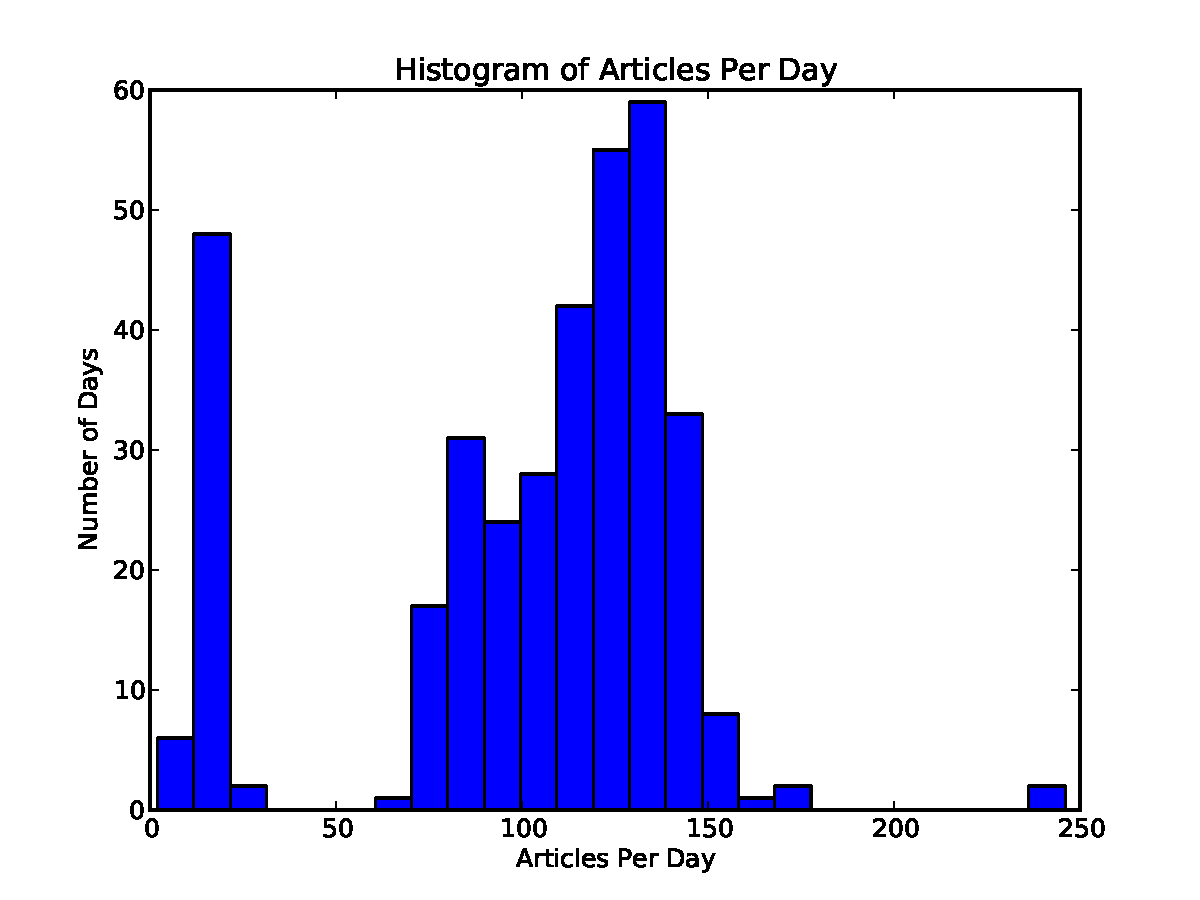
\includegraphics[scale=0.3]{text/articleshist.pdf}
\caption{Histogram of Articles Per Day}

\label{articlehist}
\end{figure}

Our data set consists of over 24 million words, with an average of 667 words per article. A histogram of article lengths appears in Figure~\ref{wordshist}. Most articles tend to be less than 2000 words, but there appears to be a long tail consisting of a few very long articles. For the most part it appears that article lengths are similar apart from a few outliers.


\begin{figure}
\centering
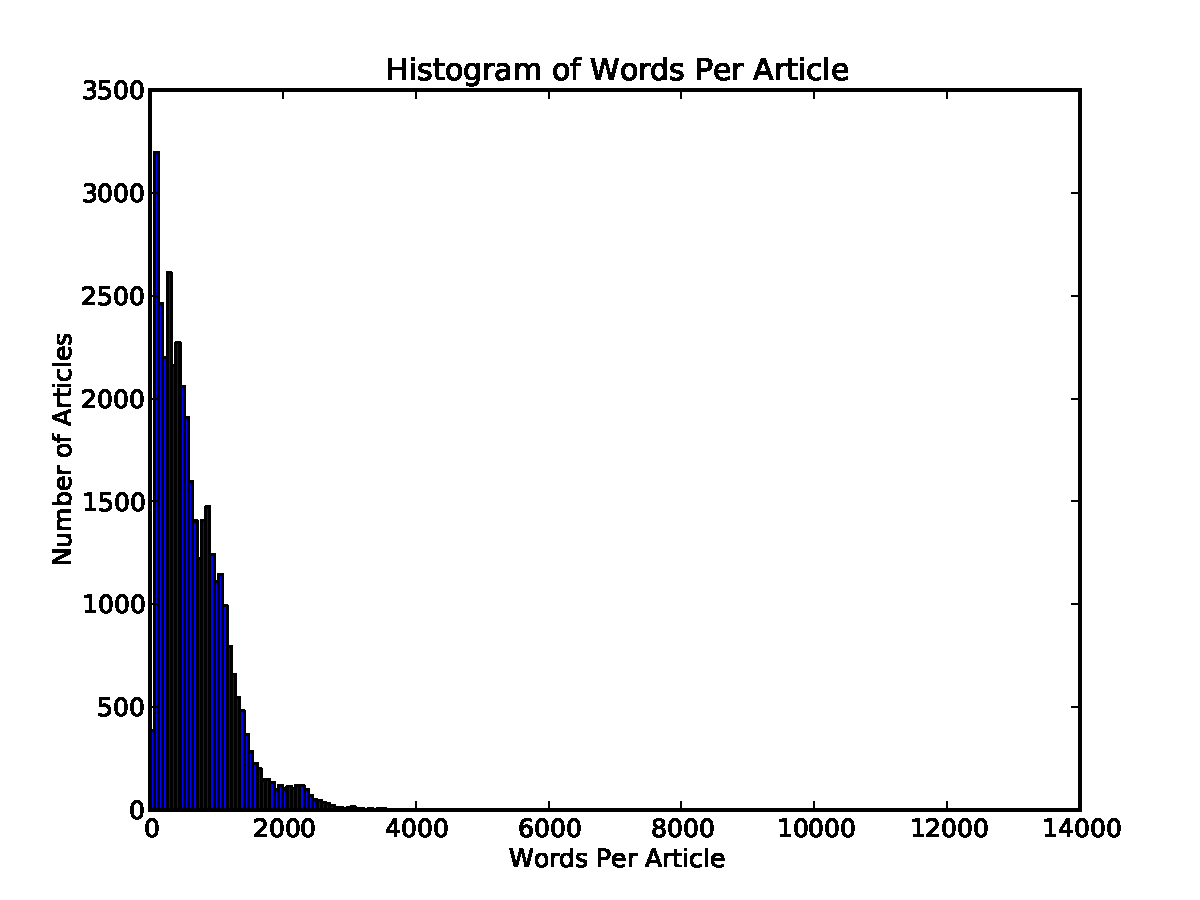
\includegraphics[scale=0.3]{text/wordshist.pdf}
\caption{Histogram of Words Per Article}
\label{wordshist}
\end{figure}

The data set contains 150,875 unique words. Each data point we use for training and validation therefore consists of a class label (+1 if the market went up that day, -1 if it went down) and a feature vector computed using frequencies of these unique words.

Due to the difficulty of computation on the number of unique words that we have, we filter the words in several ways to reduce the noise of the data set. First, we strip all non-alphabetic characters from all words and filter out any words less than length 2. We then filter out any words that did not appear more than some cutoff, $m$, throughout the year. We assume that these words are either misspellings or words which would not generally be useful in predicting stock performance due to their infrequency. Filtering with $m = 10$ results in 44,218 unique words and was found to be a good balance between information and computational tractability.
Finally, we filtered out any of the 100 most commonly used English words~\footnote{http://en.wikipedia.org/wiki/Most\_common\_words\_in\_English}, since we
assume that words such as ``and'' and ``I'' do not provide very much information.

We use several feature extraction techniques to construct the data matrix $F$. Each row of $F$ is the feature for a corresponding day, and each column of $F$
contains the values for one feature across all days. The column-vector $Y$ contains the output values (+1 or -1). 

The rest of this section describes several feature extraction techniques we used and the representation of the feature matrix $F$.  These features are compared using several machine learning algorithms presented in Section~\ref{sec:techniques}.

We will introduce the following terminology to describe the feature matrix and its elements:

\begin{itemize}


\item $F_{d,i}$ is the ith element of the feature vector for day $d$.

%\item $W$ is a vector with a count for each word over the entire year. Thus, $W_i$ is the number of times word $i$ appeared in the year.  

\item $A$ is a vector of word counts for a single article. Thus, $A_i$ is the number of times word $i$ appeared in article $A$.

\item $D$ is a vector of days, each element of which is a set of articles. $A \in D_k$ if and only if article $A$ was published on day $k$.


\end{itemize}

\subsection{Bag of Words and Phrases}

The simplest feature vector is simply a ``bag of words'' for each day~\cite{featurehash}, which consists of frequency counts of all words in articles published on that day. Elements of the feature vector take the form: $$\displaystyle F_{d,i} = \sum_{A \in D_d}{A_i}$$ These feature vectors are extremely sparse, since most articles do not use tens of thousands of unique words (we represent our data set as a sparse matrix
in MATLAB to reduce memory consumption to reasonable levels).

An obvious weakness of this technique is that it takes words out of context. Phrases such as ``stocks went up'' simply increase the counts of the three words independently. We augmented this technique by creating ``bags of phrases'' as well. In addition to counts of words, we keep counts of two and three word phrases
as well. We turn phrases into single words of the form ``word1-word2'' and ``word1-word2-word3'' with the restrictions that word1 and word3 may not be common words and the first or last words of a phrase may not be a single character. Common words beginning a 2 word phrase or ending a 3 word phrase are undesirable because we want to pick up on phrases where the subject is important. The middle word in the 3 word phrases may be common so we find phrases that combine two useful words such as, ``stocks are down.'' Filtering out phrases that appear less than $m = 10$ times in the year results in 194,679 unique phrases and words, so this technique can greatly increase the number of features.

Bags of words and bags of phrases form the basis of many of our other feature selection techniques, so we will call the feature matrix resulting from the use of either $B$. Since bags of phrases just increase the vocabulary size, it can be viewed as augmenting the article word lists $A$ with additional words. They bags of words or phrases may be used interchangeably, so we will refer to the resulting feature matrix for either as $B$ in the rest of this section; when we present results we will explicitly state if we build on bags of words or phrases as well as the filtering parameters used.

\subsection{Temporal Features}

The words and phrases from previous days may have an influence on the current day's market direction by representing trends in the market~\cite{mlstockmarket}. Building a model which takes temporal information into account may use information about these trends to make better predictions. We incorporate temporal information by augmenting our data set with data from previous days and using the resulting feature vectors for training and testing.

The first method we consider is \textit{temporal concatenation} of our bag of words. The previous $L$ days features are concatenated on to the end of the current day's feature. That is, $F_{d} = B_{d} \oplus B_{d-1} \oplus ... \oplus B_{d-L}$, where ($\oplus$) represents vector concatenation, and where days before the start of our data set are assumed to have counts $0$ for all words.

A major problem with this method is that it increases the length of our feature vectors by a factor of $L$, which quickly becomes intractable for large $L$. To use this method, we need to filter out more words from our initial data set which may reduce the information we have. Another problem with temporal concatenation is that it also includes information about which specific day in the past had each word. If the phrase ``market downturn'' is associated with decreases in the following week, then it doesn't matter if it appeared one or two days in the past. This observation is similar to that made in~\cite{mlstockmarket} in which the author assumes that certain articles may have an effect on the stock price that lingers for some time and then diminishes in importance. 

The second method we consider, which we call \textit{temporal memory}, addresses this issue. Each feature vector is augmented with a weighted average of the frequencies of each word over the previous $L$ days. That is, $$\displaystyle F_{d} = B_{d} \oplus {{\sum^L_{i=1}{\alpha_i B_{d-i}}} \over {\sum^L_{i=1}{\alpha_i}}}$$ Again, frequencies are assumed to be 0 for days before the beginning of our data set, and we round the weighted average up to an integer. This allows us to specify the relative weights of historic data for the previous $L$ days while only doubling the size of our feature vectors. 

\subsection{Topic Modeling}

The feature vectors previously described in this section are all very high-dimensional, containing either tens- or hundreds-of-thousands of word frequencies. This is problematic for several learning algorithms we applied, including SVMs and K-Nearest-Neighbor. We use dimensionality reduction and topic modeling techniques to reduce the dimensionality of the feature vectors while retaining important semantic information.

The primary technique we use is Latent Semantic Indexing~(LSI)~\cite{lsi}. The input to LSI is a term-document matrix, a matrix in which each row represents a term and each column represents a document. The element at row $t$ and column $d$ is the frequency of term $t$ in document $d$ (this is the transpose of our bag of words feature matrix $B$, viewing each day as a ``document''). LSI requires finding the Singular Value Decompositon (SVD) of this term-document matrix. If $X$ is our $t \times d$ term-document matrix, then the SVD of $X$ are the unique matrices $T, S, \text{ and } D$, such that $T$ is $t \times m$, S is diagonal $m \times m$, $D$ is $d \times m$ and $X = T S D'$, where $D'$ is the transpose of $D$. By the definition of SVD, the columns of $T$ are eigenvectors of $X X'$, the rows of $D$ are the eigenvectors of $X' X$, and $S$ is a diagonal matrix of the square roots of the eigenvalues for both. The fundamental insight used by LSI is that zeroing out all but the $r$ largest eigenvectors in $S$ results in a new matrix $\hat{X}$ which is the closest matrix of rank $r$ to the original $X$ by least-squares~\cite{lsi}. Zeroing out those elements also means we need to retain only $m$ columns of $T$ and $D$ to construct the new matrix, so we have greatly reduced the number of columns we must retain for $r << m$. This result is called the rank-reduced SVD. The $r$ columns of $D$ corresponding to the $r$ largest eigenvalues represent each document with only $r$ features, multiplying by $S$ scales this new vector space appropriately, so we use $S D'$ as our data matrix which is $d \times r$ with similarity between vectors representing similarity between semantic information in the original input space. The LSI paper recommends finding similarity by cosine of the angle between vectors, and we compare using angle and Euclidean distance in our results. New input vectors can be projected into this new space through a method described in~\cite{lsi}.

\TODO{Add figures showing features in this reduced space}

\TODO{Should we do PLSI?} 

\section{Classifiers}
\label{sec:techniques}

In this section we describe the different classifiers we developed for this project.
For each classifiers we describe our implementation choices and what, if any, third-party libraries we used.

Our classifiers can roughly be divided into four categories. The first are simple prediction rules. These are mostly included to demonstrate features of our data and to serve as baselines for the other classifiers. The next class include classifiers that do not have a probabilistic model. These include AdaBoost, Nearest Neighbor and SVM. The third class consist of classifiers based on probabilistic models. The only classifiers we implemented in this category is Naive Bayes. The fourth and final class of classifiers is sequential models and include M-order Markov Models and Hidden Markov Models.

\subsection{Naive Bayes}
\label{sec:naive-bayes}

The first classifier we implemented was Naive Bayes.
Naive Bayes is a natural choice when the input features are discrete with very high dimensionality (such as bag of words).
The reason for this is the naive bayes assumption, which asserts that the input features are independent.
This means we can turn the multinomial on the full distribution, which has $O(2^D)$ parameters into $D$ binomials with $O(D)$ parameters.
That is, $p(Y|X) \propto p(Y)p(X|Y) = p(Y)\prod_{i=1}^{D}{p(X^{(i)}|Y)}$, where $p(Y)$ is a prior on $Y$ (we will take advantage of the opportunity to put a prior on $Y$ later).

\TODO{Are the input features independent or are they independent conditioned on the class?}

Although this assumption may seem \emph{overly} naive, it has proven to work well on document classification tasks such as spam detection, which are similar to our problem.
It is also a probabilistic model, as opposed to most of our other classifiers, which means we can combine it with temporal probabilistic models.

\subsection{AdaBoost}
\label{sec:adaboost}

The next classifier we implemented was AdaBoost using decision stumps as weak learners.
Our implementation of AdaBoost is parameterized by $M$, which denotes the number of classifiers to train.

The reason why we choose AdaBoost is that we have a very large corpus of words and need classifiers that can be trained very quickly.
Weak learners fit this bill since they can be trained in linear time in the dimensionality of the features and in the number of data points.
However, since decision stumps are terrible classifiers we boost them with AdaBoost, which makes them quite effective classifiers.
Moreover, in addition to serving as a efficient classifier on bags of words, AdaBoost helps us gain insight into our data set as the training picks out the words that does the best job of separating the dataset.

\subsection{Nearest Neighbor}
\label{sec:nearest-neighbor}

\TODO{Chris: Write this section.}

\subsection{SVM}
\label{sec:svm}

\TODO{Chris: Write this section. Say that we chose SVM's since they are probably the most popular classifiers due to their efficiency. However, we could not possible train them on the bag of words, so their usage necessitated dimensionality reduction.}

\subsection{Sequential Models}
\label{sec:sequential-models}

Stock Markets are known to follow trends and previous results are an often an indication of future results.
Therefore, we experimented with two sequential models to attempt to predict the Dow Jones based on past performance.

The basic versions of these models only use the previous history of Dow Jones performance to predict future results, and ignores the issues of the Wall Street Journal.
However, we also combined Hidden Markov models with Naive Bayes in an attempt to improve our predictions by taking more information into account.

\subsubsection*{Markov Models}
\label{sec:}

We implemented M-order Markov Models for any value of M. However, since the number of model parameters grows exponentially in M, we are restricted to relatively small values of M by computational resources.

\subsubsection*{Hidden Markov Models}
\label{sec:}

We also implemented a classifier for the more powerful Hidden Markov Models. An HMM assumes the observed values $Y$ are generated from a sequence of hidden states $Z$.
The evolution of the hidden states is governed by the conditional probability distribution $p(Z_{i}|Z_{i-1})$ and the values of $Y_{i}$ are governed by the conditional probability distribution $p(Y_{i}|Z_{i})$.
This is depicted graphically as a Bayes Net in figure~\TODO{ref}.

The HMM classifier is trained using the first $t$ values of $Y$ and then used to predict value $T_{t+1}$.
We used the MATLAB HMM Toolkit to learn the maximum-likelihood estimation of the model parameters A (the transition matrix) and B (the emission matrix) using the hmmtrain function, which internally uses the EM algorithm.
We then used the function hmmdecode to generate the posterior probability on state $Z_{t}$.
We then performed standard message passing along the chain from $Z_{t}$ to $Y_{t+1}$ to evaluate the marginal $p(Y_{t+1})$, which we used to predict the next value of $Y$ (see figure~\TODO{ref}).

In a variation on this approach we combined the Hidden Markov Model with Naive Bayes to make prediction both based on trends in the market and based on the articles in the Wall Street Journal.
To do this we first evaluated the marginal $p(X_{t+1})$ as described above.
We then trained a Naive Bayes predictor on the first $t$ (X,Y) tuples and used this to predict the value of $X_{t+1}$, using marginal $p(X_{t+1})$ from the HMM as a prior.
That is, we combine our prior belief about which way we think the market will go based on recent performance, with the new information in the WSJ.
This is illustrated in figure~\TODO{ref}. 


\section{Analysis}

\subsection{Temporal Shift}


Temporal shifting trades information about the current day for information about the previous (or next) day.


The bag features $B$ associate each day's price direction in $Y$ with the same day's article counts, so we are using that feature matrix to find a correlation between the direction of the stock market and the contents of newspaper articles on day $d$ (perhaps investors read the paper in the morning and that influences their trades, or some hidden ``state of the market'' influences both). It is plausible, however, that the articles on day $d-1$ are correlated with the market direction on day $d$. It is also likely that the articles on day $d+1$ are correlated with the market direction on day $d$, since they may reflect on market performance for the previous day. This is an uninteresting predictor, but it will give us some indication of how well the techniques we apply make predictions based on data that has a clear reason for being correlated.

We introduce temporally shifted feature matrices to investigate these possibilities, defined by $F_{d,i} = B_{d-1,i}$ and $F_{d,i} = B_{d+1,i}$ That is, each count is replaced either by the previous day's count or the next day's count. The first and last days' counts will be 0 respectively, so this loses some information for one day each.

\begin{itemize}
\item The word ``ambitions'' is the best indicator of the Dow Jones gaining. If ``ambitions'' appeared in the WSJ there was a 64.26\% chance that the Dow Jones went up on that day.
\item The word ``tundra'' is the best indicator of the Dow Jones falling. If ``tundra'' appeared in the WSJ there was a 64.26\% chance that the Dow Jones fell on that day. This is because a series of articles in the WSJ where they talk about how Toyota is producing more cars outside the us and where they mention the Toyota Tundra. Another item is how Toyota is passing GM in sales (tundra is mentioned). A third item is about how Tundras had to be discounted (Toyota is on the Dow Jones).

\end{itemize}

\bibliographystyle{plain}
\bibliography{report.bib}

\end{document}
